% LaTeX file for resume 
% This file uses the resume document class (res.cls)

\documentclass{res} 
%\usepackage{helvetica} % uses helvetica postscript font (download helvetica.sty)
%\usepackage{newcent}   % uses new century schoolbook postscript font 
\setlength{\textheight}{9.5in} % increase text height to fit on 1-page 
\usepackage{graphicx}
\usepackage{wrapfig}

\begin{document}
 


\name{NITHIN THILAKAPPAN\\[12pt]}     % the \\[12pt] adds a blank
				             

\address{\bf  ADDRESS\\106, Radhe Krishna Appt.,\\Opp. Patel Petrol pump\\Amli, Silvassa\\D\&NH 396230}
\address{\bf CONTACT \\ Mo. : +91 9737191961 \\  E-mail:tnithin28@gmail.com }


                                                         
\begin{resume}
\begin{figure}[h]
\centering
%\begin{wrapfigure}{r}{1in}
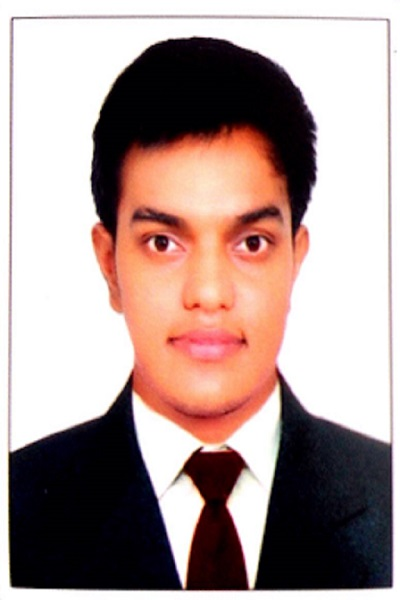
\includegraphics[width=0.2\textwidth, height=0.15\textheight]{photo}
%\end{wrapfigure}
\end{figure}

\section{OBJECTIVE}          
Looking for an organization that offers challenging and learning environment which recognize and utilize my true potential while nurturing my technical skills.


 
\section{EDUCATION}  
\begin{itemize}
\item Pursuing 8th Semester Bachelor of Engineering (Electrical Engineering)
\end{itemize}    
    
    \begin{table}[ht] 
 \centering% used for centering table
\begin{tabular}{c c c c c} % centered columns (4 columns)
\hline\\ [1ex] %inserts double horizontal lines
EXAMINATION & BOARD/UNIVERSITY & INSTITUTE/SCHOOL & YEAR & RESULT/CGPA \\ [1ex] % inserts table
%heading
\hline\\ [.5ex]% inserts single horizontal line
BE & GTU & Vadodara Institute of Engg. & 2018 & 7.17 \\ [.5ex] % inserting body of the table
HSC & GSHEB & Prabhat Scholar's Academy & 2014 & 61 \\ [.5ex] %
SSC & GSEB & Prabhat Scholar's Academy & 2012 & 70 \\ [1ex]
\hline %inserts single line 
\end{tabular}
\label{table:lin} % is used to refer this table in the text
\end{table}

\section{PROJECT}
\begin{itemize}\itemsep -2pt  % reduce space between items
\item Name: Automatic Stirrup Making Machine
\item During: Sem 7 \& 8
\item Description: The project was undertaken to study and design a model of automatic stirrups making machine using Programmable Logic Controller (PLC), which will change the conventional practices of cutting and bending the rod to make stirrups of different size and various shapes. It can reduce a lot of labour cost; human effort and construction lead time and also acquires accuracy and precision which have not been achieved in the conventional way.
\item Responsibility:-
\begin{enumerate}
\item Hardware implementation 
\item Interfacing of AC servo motor, rotary encoder, HMI \& sensors with the PLC
\item Documentation
\end{enumerate}
\end{itemize}
 
\section{TECHNICAL SKILLS}
\begin{itemize}\itemsep -2pt  % reduce space between items
\item Instrumentation and Electrical measurements
\item Electrical Wiring
\item PLC Programming
\item HMI designing
\item Machines Operation \& Installation
\item Circuit Fault Solving

\end{itemize}   

\section{SOFTWARE SKILLS}
\begin{itemize}
\item GX works3 PLC Programming Software
\item GT designer3 HMI Desgning Software
\item Bascom AVR - MCS Electronics
\item Eagle - Circuit Designing Software
\item Proteus Simulation Software
\end {itemize}


\section{SOFT SKILLS}          
    \begin{itemize} \itemsep -2pt  % reduce space between items
\item Strong analytical and people management skills.
\item Accuracy and Attention to details. 
\item Experience in working as part of a multidisciplinary research team.
\item Excellent time manager with the ability to work independently.
\item Passion for constant improvement.
\item Ability to make sound decisions.
\item Excellent organization and prioritization skills.
 \end{itemize}

\section{TRAINING/INTERNSHIP}          
\begin{itemize} \itemsep -2pt  % reduce space between items
\item Attended an Industrial training \& Internship at “MITSUBISHI ELECTRIC INDIA PRIVATE LIMITED” in Oct 2017             
 \item Successfully completed the training course in the following: -
\begin{enumerate}
\item PLC
\item HMI
\item VFD
\item SERVO                
\end{enumerate}
\end{itemize}

 
\section{INDUSTRIAL VISITS}  
\begin{itemize} \itemsep -2pt  % reduce space between items
\item  Gujarat Industries Power Company Ltd.(GIPCL), Surat
\item Gujarat State Electricity Corporation Ltd. (GSECL), Sikka
\item Gujarat Urja Vikas Nigam Ltd, Surat
\item Mitsubishi Electric India Pvt Ltd, Ahemdabad
\item Nuclear  Power  Plant, Kakrapar   
\end{itemize}

\section{CO-CURRICULAR ACTIVITIES}  
\begin{itemize} \itemsep -2pt  % reduce space between items
\item Participated in national competition \textbf {Mitsubishi Electric Cup 2018} held at Nirma University, Ahmedabad on February 2018 
\item Participated in \textbf {National ABU Robocon 2018} held at Pune in March 2018.
\item Participated  in National level competition \textbf {World Robotic Olympaid (Advance Robotic \\Category)} held at Delhi in October 2017.
\item Participated in \textbf {National ABU Robocon 2017} held at Pune in March 2017.
\item  Participated in Robotics Competition (Line Follower Robot) on the theme \textbf {“Make in India”} under the banner of \textbf {ISTE (Indian Society for Technical Education)} Gujarat section held at Rajkot, in October 2016.   
\item  Participated in \textbf {“National Robocon 2016”} held at Pune in March 2016.
\item Certificate of participation in workshop on \textbf {Energy Conservation Awareness Program} organized by Gujarat Energy Development Association(GEDA) in September 2017.
\item Certificate of participation in workshop on \textbf {Embedded System} organized by \textbf {Smartec\\ Solutions} Vadodara in July 2017 
\item Certificate of participation in technical event \textbf {GTU Techfest (Electric loot)} held at L.D. College of Engineering, Ahmedabad in March 2017.
\item Certificate of participation in \textbf {Robotics} and \textbf {Circuit Solution} competition on the theme \textbf{“Make in India”} under the banner of ISTE (Indian Society for Technical Education) Gujarat section held at Rajkot, in Oct 2016.
\item Certificate of participation in National level technical symposium \textbf{Prakarsh} held at Saradar Vallabhbhai Institute of Technology(SVIT) Vasad in February 2016.
\item Certificate of participation in technical event \textbf {GTU Techfest (S.M.I.L.E)} held at L.D. College of Engineering, Ahmedabad in March 2015.
\end{itemize}
        


\section{ACHIEVEMENTS}
\begin{itemize}\itemsep -2pt  % reduce space between items
\item  Winner of National level competition \textbf {eYantra Ideas Competition (eYIC-2018)} \\  Awarded with \textbf{Best Demonstration \& Presentation Award and  Best Judge’s Choice Award } at IIT Bombay in April 2018.

\item 7th position in all over India in the National competition \textbf {Mitsubishi Electric Cup 2018} held at Nirma University, Ahmedabad on February 2018 
\item Winner in national level competition \textbf {World Robotic Olympaid (Advance Robotic Category)} held at Delhi in October 2017.
\item 2nd Runner up in\textbf {National ABU Robocon 2017} held at Pune in March 2017.
\item Winner in \textbf {Robotics Competition (Line Follower Robot)} on the theme \textbf {Make in India} under the banner of ISTE (Indian Society for Technical Education) Gujarat section held at Rajkot, in October 2016.   
\item Winner in \textbf {National ABU Robocon 2016} held at Pune in March 2016.
\item Best Design Award in \textbf {International ABU Robocon 2016} held at Bangkok, Thailand in August 2016.

\end{itemize}
\section{ Personal Details}

 Father's Name: Thilakappan\\ [0.5ex]
 Mother's Name: Sudharma Thilakappan \\ [0.5ex]
 Sex: Male\\ [0.5ex]
 Date of Birth: 28 November 1996\\ [0.5ex]
 Nationality: Indian\\ [0.5ex]
 Marital Status: Unmarried\\ [0.5ex]

\section{References}

\begin{enumerate}

\item Dr. Jayeshkumar S. Patel\\
\ Principal\\
\ Vadodara Institute of Engineering\\
\ Vadodara\\
\ Contact number: 02653915900\\
\ Email: vierorgin@yahoo.com\\

\item Prof. Ujjaval Patel\\
\ Head of Department\\
\ Vadodara Institute of Engineering\\
\ Vadodara\\
\ Mobile: +917984310785\\
\ Email: ujjaval58@rediffmail.com\\


\item Prof. Satish Bhati\\
\ Assistant professor\\
\ Vadodara Institute of Engineering\\
\ Vadodara\\
\ Mobile: +919909959321\\
\ Email: bhatisatish4045@gmail.com\\

\end{enumerate}

\section{Declaration}
 I hereby declare that the above mentioned information is true to the best of my knowledge.

\section{Date}
19/04/2018 
 

\end{resume}
\end{document}